%========================================================
\chapter{System Design and Architecture}
%========================================================
The design of the proposed Trade-Based Money Laundering detection framework focuses on developing a scalable, privacy-preserving, and intelligent financial monitoring system capable of analyzing complex transactional relationships within large-scale trade ecosystems. Since modern TBML activities involve interconnected financial entities, cross-border transactions, and evolving laundering strategies, the system architecture must support efficient graph-based analysis, real-time monitoring, and secure institutional collaboration. This chapter discusses the major design considerations, overall system architecture, module-level organization, and data flow mechanisms associated with the proposed fraud detection framework.

%========================================================
\section[Design Considerations]{\textbf{Design Considerations}}
%========================================================

The design of the proposed TBML detection framework is influenced by multiple operational, analytical, and security-related factors associated with large-scale financial monitoring systems. Since Trade-Based Money Laundering activities involve interconnected financial entities, cross-border transactions, and hidden transactional relationships, the system architecture must support efficient graph-based representation and relational analysis of financial data. The framework is therefore designed to support scalable transaction monitoring and fraud analysis within distributed institutional environments.

Security and privacy preservation also represent important considerations in the proposed system design. Financial institutions operate under strict regulatory policies that restrict unauthorized access and direct sharing of sensitive transactional information. Consequently, the framework incorporates secure authentication mechanisms, role-based access control, and federated learning strategies to support protected institutional collaboration and privacy-preserving analytical processing.

The proposed framework is additionally designed using a modular architecture to simplify system integration, maintenance, and future scalability. Individual modules associated with transaction monitoring, graph construction, fraud detection, compliance reporting, and dashboard visualization operate independently while maintaining coordinated interaction within the overall monitoring environment.


%========================================================
\section[Overall System Architecture]{\textbf{Overall System Architecture}}
%========================================================

The overall architecture of the proposed TBML detection framework is designed to support intelligent financial transaction monitoring, graph-based fraud analysis, federated learning, and automated compliance reporting within distributed institutional environments. The framework integrates transaction processing services, heterogeneous graph construction mechanisms, machine learning-based fraud detection modules, and real-time monitoring interfaces to identify suspicious transactional relationships associated with Trade-Based Money Laundering activities.

The architecture begins with multiple input systems including banking systems, trade systems, and external financial data sources. Raw transactional information, trade-related documents, KYC records, and institutional monitoring logs are initially processed within the transaction processing module. This stage performs stream ingestion, validation, cleansing, normalization, and structured event generation to prepare financial data for analytical processing.

The processed transactional data is subsequently transformed into heterogeneous graph structures within the graph construction module. Financial entities such as accounts, organizations, transactions, invoices, and trade relationships are represented as interconnected nodes and edges to capture hidden financial dependencies and suspicious transactional patterns. The generated graph data consists of node features, edge relationships, and graph connectivity information required for graph-based machine learning operations.

The fraud detection layer incorporates a Hybrid Graph Neural Network branch for relational analysis and a temporal learning branch for capturing sequential transactional behavior. These analytical modules process the generated graph structures and institutional transaction sequences to learn complex laundering patterns associated with suspicious financial activities. The outputs generated from the analytical models are combined to improve fraud representation learning and transaction risk prediction accuracy.

To preserve institutional privacy and regulatory compliance, the proposed framework integrates a federated learning environment in which participating institutions perform localized model training without directly sharing sensitive financial information. Local model updates generated at institutional environments are transmitted to the global aggregation module, where the updates are combined to construct an improved global fraud detection model while maintaining privacy-preserving collaborative learning.

The updated global model is utilized within the inference and risk scoring module to classify suspicious financial transactions and generate fraud risk scores. Transactions identified as potentially suspicious are forwarded to the compliance management environment for alert generation, Suspicious Transaction Report creation, and regulatory integration support. The overall architecture of the proposed TBML detection framework is illustrated in Figure~\ref{fig:overall_architecture}.

\begin{figure}[H]
    \centering
    \fbox{
        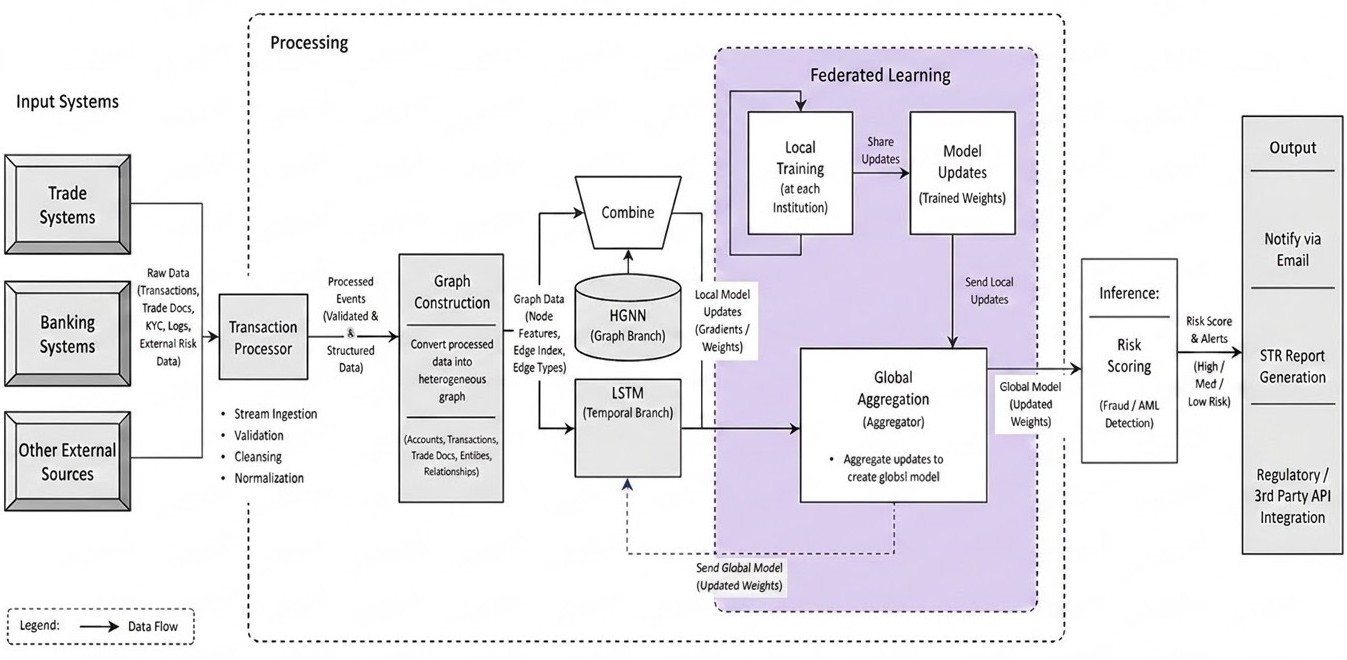
\includegraphics[width=0.98\textwidth]{Figures/overall_architecture.jpg}
    }
    \caption{Overall Architecture of the Proposed TBML Detection Framework}
    \label{fig:overall_architecture}
\end{figure}

%========================================================
\section[Module Design]{\textbf{Module Design}}
%========================================================

%========================================================
\subsection[Authentication and Access Control Module]{\textbf{Authentication and Access Control Module}}
%========================================================


%========================================================
\subsection[Transaction Monitoring Module]{\textbf{Transaction Monitoring Module}}
%========================================================


%========================================================
\subsection[Graph Construction Module]{\textbf{Graph Construction Module}}
%========================================================


%========================================================
\subsection[Graph Neural Network Fraud Detection Module]{\textbf{Graph Neural Network Fraud Detection Module}}
%========================================================


%========================================================
\subsection[Federated Learning Coordination Module]{\textbf{Federated Learning Coordination Module}}
%========================================================


%========================================================
\subsection[Suspicious Transaction Report Generation Module]{\textbf{Suspicious Transaction Report Generation Module}}
%========================================================


%========================================================
\subsection[Dashboard Visualization Module]{\textbf{Dashboard Visualization Module}}
%========================================================


%========================================================
\section[Data Flow Diagrams]{\textbf{Data Flow Diagrams}}
%========================================================

%========================================================
\subsection[Data Flow Diagram Level 0]{\textbf{Data Flow Diagram Level 0}}
%========================================================


%========================================================
\subsection[Data Flow Diagram Level 1]{\textbf{Data Flow Diagram Level 1}}
%========================================================


%========================================================
\subsection[Data Flow Diagram Level 2]{\textbf{Data Flow Diagram Level 2}}
%========================================================


%========================================================
\section*{Summary}
%========================================================